\documentclass[10pt,mathserif]{beamer}
\usepackage[T5]{fontenc}
\usepackage[utf8]{inputenc}
\usepackage{graphicx,amsmath,amssymb,tikz,psfrag}

\input defs.tex

%% formatting

\mode<presentation>
{
\usetheme{default}
}
\setbeamertemplate{navigation symbols}{}
\usecolortheme[rgb={0.13,0.28,0.59}]{structure}
\setbeamertemplate{itemize subitem}{--}
\setbeamertemplate{frametitle} {
	\begin{center}
	  {\large\bf \insertframetitle}
	\end{center}
}

\newcommand\footlineon{
  \setbeamertemplate{footline} {
    \begin{beamercolorbox}[ht=2.5ex,dp=1.125ex,leftskip=.8cm,rightskip=.6cm]{structure}
      \footnotesize \insertsection
      \hfill
      {\insertframenumber}
    \end{beamercolorbox}
    \vskip 0.45cm
  }
}
\footlineon

\AtBeginSection[] 
{ 
	\begin{frame}<beamer> 
		\frametitle{Outline} 
		\tableofcontents[currentsection,currentsubsection] 
	\end{frame} 
} 

%% begin presentation

\title{\large \bfseries Gesture Generation}

\author{Thanh Hoang-Minh\\[3ex]
University of Science}

\date{\today}

\begin{document}

\frame{
\thispagestyle{empty}
\titlepage
}

\section{Sinh cử chỉ}

\begin{frame}
\frametitle{Bulleted list}
\begin{itemize}\itemsep=12pt
\item XXX
\vspace*{0.5em}
\begin{itemize}
\item XXX
\item XXX
\item XXX
\end{itemize}
\item XXX
\vspace*{0.5em}
\begin{itemize}
\item XXX
\item XXX
\item XXX
\end{itemize}
\item XXX
\end{itemize}
\end{frame}

\begin{frame}
\frametitle{Pictures with tikz}
\begin{center}
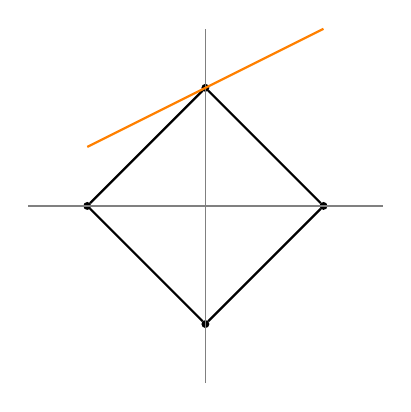
\begin{tikzpicture}
	[scale=1.5,dot/.style={circle,draw=black!100,fill=black!100,thick,inner sep=0pt,minimum size=2pt}]
    \node[dot] at (-1,0) (n1) {};
    \node[dot] at (0,1)  (n2) {};
    \node[dot] at (1,0)  (n3) {};
    \node[dot] at (0,-1) (n4) {};
    \draw[gray] (-1.5,0) -- (1.5,0);
    \draw[gray] (0,-1.5) -- (0,1.5);
    \draw[black,thick] (n1) -- (n2) -- (n3) -- (n4) -- (n1) -- cycle;
    \draw[orange,thick] (-1,0.5) -- (0,1) -- (1,1.5);
\end{tikzpicture}
\qquad
\begin{tikzpicture}
	[scale=1.5,dot/.style={circle,draw=black!100,fill=black!100,thick,inner sep=0pt,minimum size=2pt}]
    \draw[gray] (-1.5,0) -- (1.5,0);
    \draw[gray] (0,-1.5) -- (0,1.5);
    \draw[black,thick] (-1,1) -- (0,0) -- (1,1);
\end{tikzpicture}
\end{center}
\end{frame}

\begin{frame}
\frametitle{Pictures with tikz}
\begin{itemize}\itemsep=12pt
	\item convex envelope of (nonconvex) $f$ is the largest convex underestimator $g$
    \item \ie, the best convex lower bound to a function
        \vspace*{1em}
\begin{center}
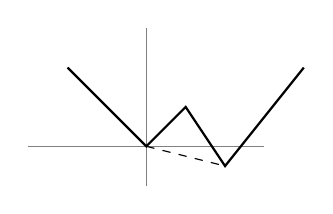
\begin{tikzpicture}
    \draw[gray] (-1.5,0) -- (1.5,0);
    \draw[gray] (0,-0.5) -- (0,1.5);
    \draw[black,thick] (-1,1) -- (0,0) -- (0.5,0.5) -- (1,-0.25) -- (2,1);
    \draw[black,dashed] (0,0) -- (1,-0.25);
\end{tikzpicture}
\end{center}
    \item \textbf{example}: $\ell_1$ is the envelope of $\card$ (on unit $\ell_\infty$ ball)
    \item \textbf{example}: $\|\cdot\|_*$ is the envelope of $\rank$ (on unit spectral norm ball)
    \item various characterizations: \eg, $f^{**}$ or convex hull of epigraph
\end{itemize}
\end{frame}

\section{Second section}

\begin{frame}
\frametitle{Group lasso \\[-0.3em] 
{\footnotesize \textmd{(\eg, Yuan \& Lin; Meier, van de Geer, B\"uhlmann; Jacob, Obozinski, Vert)}}}
\begin{itemize}\itemsep=12pt
\item problem:
\[
\begin{array}{ll}
\mbox{minimize} & f(x) + \lambda \sum_{i=1}^N \|x_i\|_2
\end{array}
\]
\ie, like lasso, but require groups of variables to be zero or not
\item also called $\ell_{1,2}$ mixed norm regularization
\end{itemize}
\end{frame}

\begin{frame}{Structured group lasso \\[-0.3em] 
{\footnotesize \textmd{(Jacob, Obozinski, Vert; Bach et al.; Zhao, Rocha, Yu; \dots)}}}
\begin{itemize}\itemsep=12pt
\item problem:
\[
\begin{array}{ll}
\mbox{minimize} & f(x) + \sum_{i=1}^N \lambda_i \|x_{g_i}\|_2
\end{array}
\]
where $g_i \subseteq [n]$ and $\mathcal G = \{g_1, \dots, g_N\}$
\item like group lasso, but the groups can overlap arbitrarily
\item particular choices of groups can impose `structured' sparsity
\item \eg, topic models, selecting interaction terms for (graphical) models,
    tree structure of gene networks, fMRI data
\item generalizes to the \textbf{composite absolute penalties family}:
\[
r(x) = \|(\|x_{g_1}\|_{p_1}, \dots, \|x_{g_N}\|_{p_N})\|_{p_0}
\]
\end{itemize}
\end{frame}

\begin{frame}{Structured group lasso \\[-0.3em] 
{\footnotesize \textmd{(Jacob, Obozinski, Vert; Bach et al.; Zhao, Rocha, Yu; \dots)}}}
\textbf{hierarchical selection}:
\begin{center}
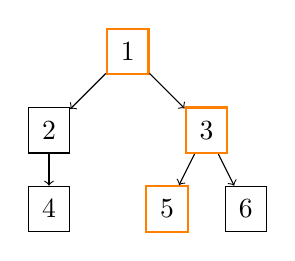
\begin{tikzpicture}
[dot/.style={rectangle,draw=black,fill=white,inner sep=5pt,minimum size=5pt}]
\node[dot,draw=orange,thick] at (0,5) (n1) {1};
\node[dot] at (-1,4) (n2) {2};
\node[dot,draw=orange,thick] at (1,4) (n3) {3};
\node[dot] at (-1,3) (n4) {4};
\node[dot,draw=orange,thick] at (0.5,3) (n5) {5};
\node[dot] at (1.5,3) (n6) {6};
\draw[->] (n1) -- (n2);
\draw[->] (n1) -- (n3);
\draw[->] (n2) -- (n4);
\draw[->] (n3) -- (n5);
\draw[->] (n3) -- (n6);
\end{tikzpicture}
\end{center}
\begin{itemize}\itemsep=8pt
    \item $\mathcal G = \{ \{4\}, \textcolor{orange}{\{5\}}, \{6\}, \{2,4\}, 
        \textcolor{orange}{\{3,5,6\}}, \textcolor{orange}{\{1,2,3,4,5,6\} \}}$
\item nonzero variables form a rooted and connected subtree
    \begin{itemize}
        \item if node is selected, so are its ancestors
        \item if node is not selected, neither are its descendants
    \end{itemize}
\end{itemize}
\end{frame}

\begin{frame}[fragile]{Sample ADMM implementation: lasso}
\begin{verbatim}
prox_f = @(v,rho) (rho/(1 + rho))*(v - b) + b;
prox_g = @(v,rho) (max(0, v - 1/rho) - max(0, -v - 1/rho));

AA = A*A';
L  = chol(eye(m) + AA);

for iter = 1:MAX_ITER
    xx = prox_g(xz - xt, rho);
    yx = prox_f(yz - yt, rho);

    yz = L \ (L' \ (A*(xx + xt) + AA*(yx + yt)));
    xz = xx + xt + A'*(yx + yt - yz);
  
    xt = xt + xx - xz;
    yt = yt + yx - yz;
end
\end{verbatim}
\end{frame}

\begin{frame}{Figure}
	\begin{center}
		\psfrag{k}[t][b]{$k$}
		\psfrag{fbest - fmin}[b][t]{$f_\mathrm{best}^{(k)} - f^\star$}
		\psfrag{noise-free realize}{noise-free case}
		\psfrag{realize1}{realization 1}
		\psfrag{realize2}{realization 2}
		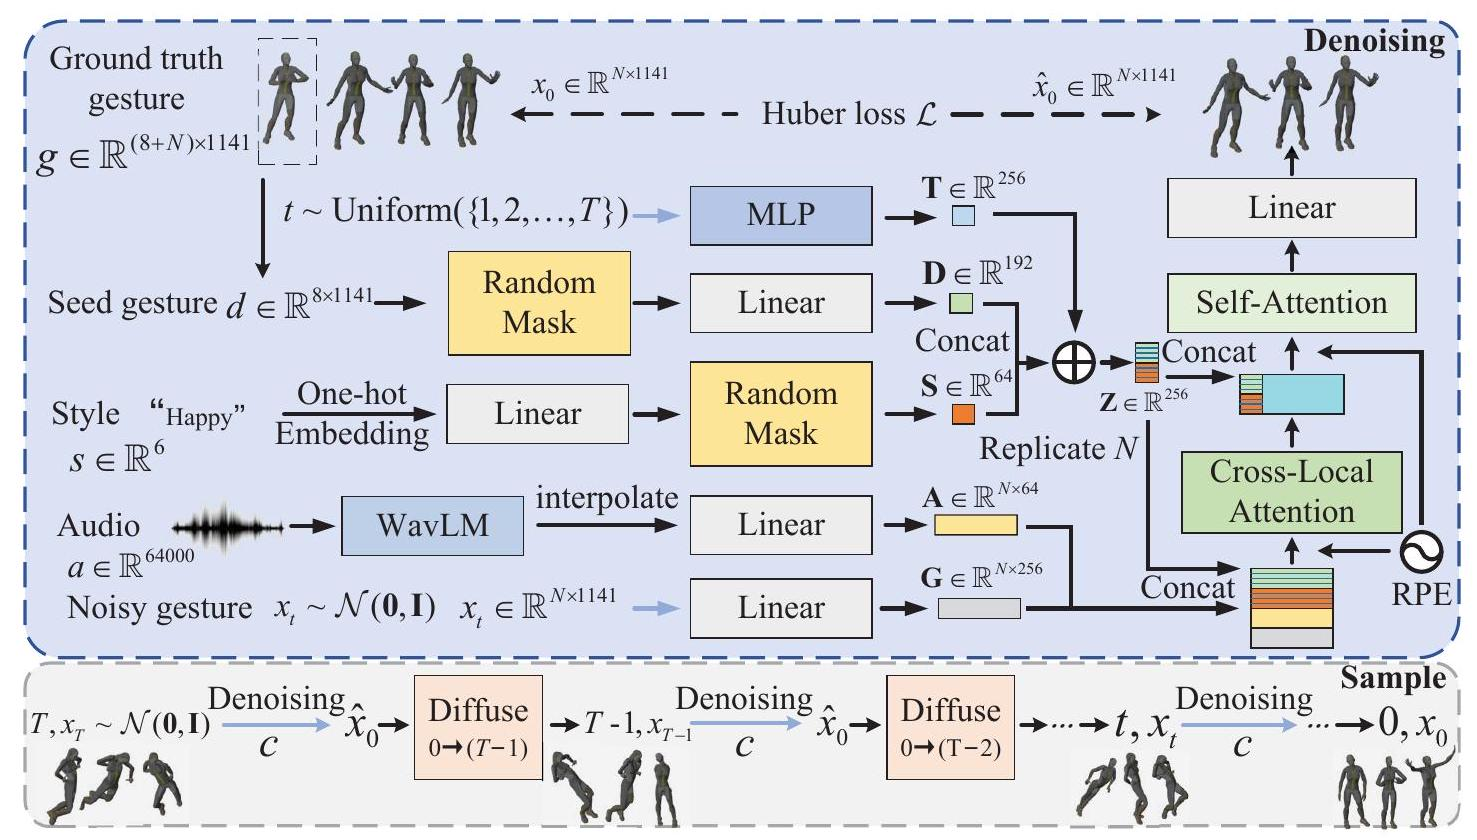
\includegraphics[width=0.8\textwidth]{figures/architecture.jpg}
	\end{center}
\end{frame}

\begin{frame}{Algorithm}
    if $L$ is not known (usually the case), can use the following line search:
    \noindent\rule[-5pt]{\textwidth}{0.4pt}
    {\footnotesize
    \begin{tabbing}
        {\bf given} $x^k$, $\lambda^{k-1}$, and parameter $\beta \in (0,1)$. \\*[\smallskipamount]
        Let $\lambda := \lambda^{k-1}$. \\*[\smallskipamount]
        {\bf repeat} \\
        \qquad \= 1.\ Let $z := \prox_{\lambda g}(x^{k} - \lambda \nabla f(x^{k}))$. \\
        \> 2.\ {\bf break if} $f(z) \leq \hat{f}_{\lambda}(z, x^{k})$. \\
        \> 3.\ Update $\lambda := \beta \lambda$. \\*[\smallskipamount]
        {\bf return} $\lambda^{k} := \lambda$, $x^{k+1}:=z$.
    \end{tabbing}}
    \noindent\rule[10pt]{\textwidth}{0.4pt}

    typical value of $\beta$ is $1/2$, and 
    \[
    \hat{f}_\lambda(x,y) = f(y) + \nabla f(y)^T (x - y) + 
    (1/2\lambda)\|x - y\|_2^2
    \]
\end{frame}


\end{document}
